\begin{frame}
\begin{center}
    \Large
    Life Cycle Assessment - Overview
\end{center}
\end{frame}

\begin{frame}{Life Cycle Assessment - Overview}
\begin{figure}
    \centering
    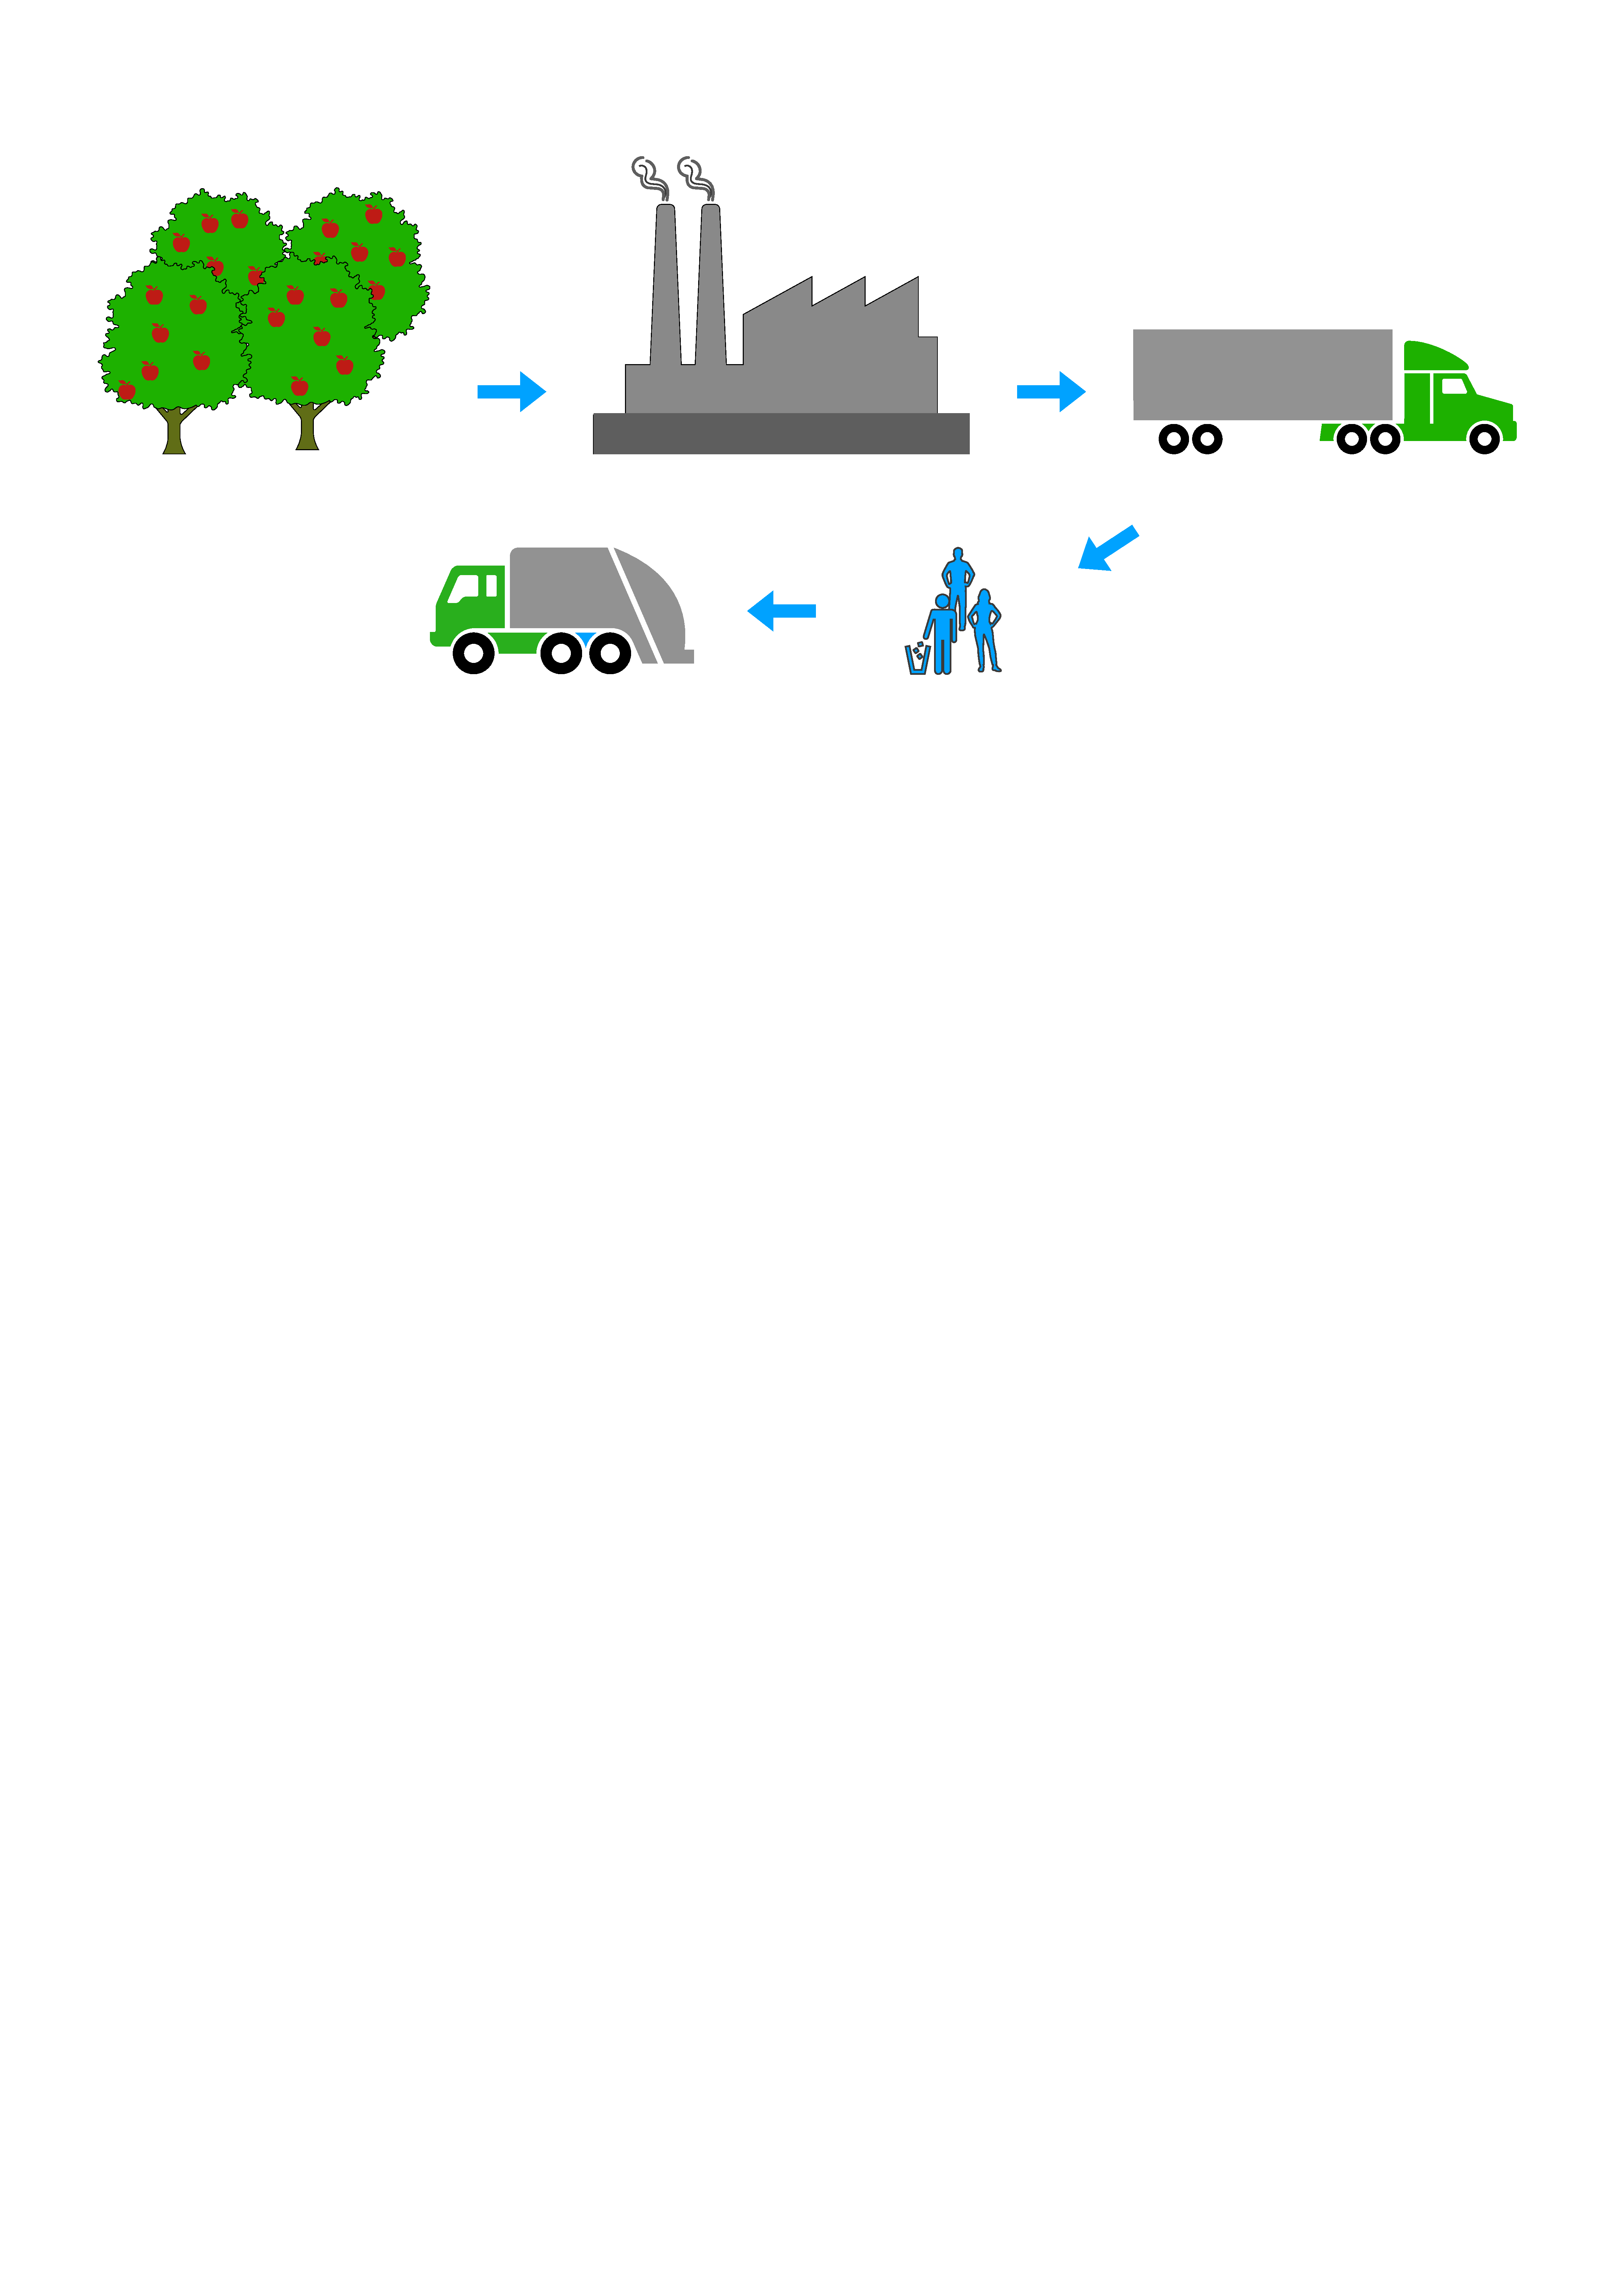
\includegraphics[width = 0.7\linewidth]{.figures/AppleJuiceExample.pdf}
    \caption{Apple juice production system example.}
\end{figure}
\end{frame}

\begin{frame}{Life Cycle Assessment - Overview}
Four phases of LCA:
\begin{enumerate}
    \item Goal and Scope
    \item Life Cycle Inventory (LCI)
    \item Life Cycle Impact Assessment (LCIA)
    \item Interpretation
\end{enumerate}
\end{frame}

\begin{frame}{Life Cycle Assessment - Overview}
\begin{figure}
    \centering
    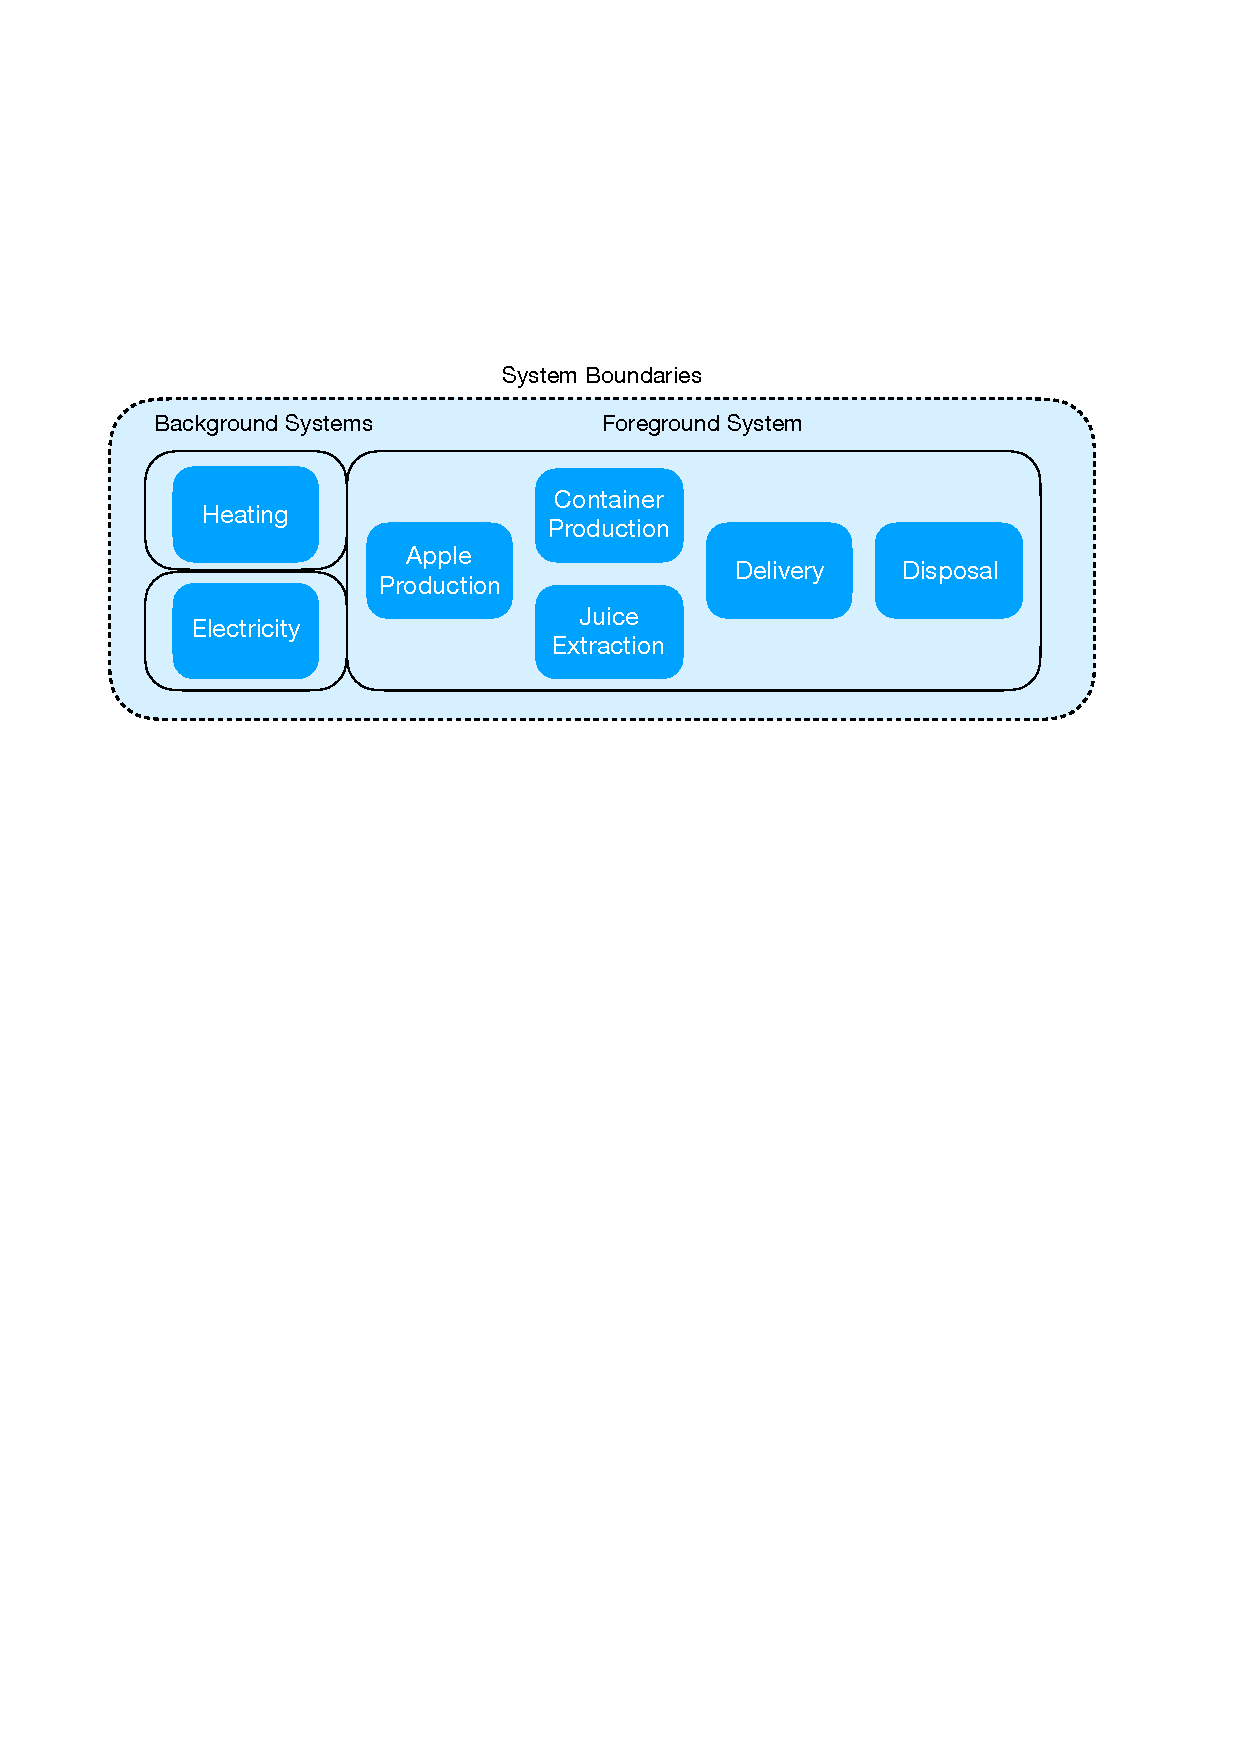
\includegraphics[width=1\linewidth]{.figures/InventoryComponents.pdf}
    \caption{LCI components for apple juice production}
\end{figure}
\end{frame}

\begin{frame}{Life Cycle Assessment - Overview}
From \textit{Life Cycle Assessment - Theory and Practice}:
\begin{center} \color{darkgray}
    \textit{"Calculate LCIA results per impact category:\\ 
    For each impact category separately, calculate the LCIA indicator results by multiplying the amount of each contributing (i.e. classified) elementary flow of the inventory with its characterisation factor. The results may be summed up per impact category, but summing up shall not be done across impact categories"}
\end{center}
\end{frame}

\newcommand{\red}[1]{{\color{red}#1}}
\begin{frame}{Life Cycle Assessment - Overview}
From \textit{Life Cycle Assessment - Theory and Practice}:
\begin{center} \color{darkgray}
    \textit{"Calculate LCIA results per impact category:\\ 
    For each impact category separately, calculate the LCIA indicator results by \red{multiplying} the amount of each contributing (i.e. classified) \red{elementary flow} of the inventory with its \red{characterisation factor}. The results may be \red{summed up per impact category}, but summing up shall not be done across impact categories"}
\end{center}
\end{frame}